% Capítulo 3
\chapter{Proposta}
\label{proposta}

%%%%%%%%%%%%%%%%%%%%%%%%%%%%%%%%%%%%%%%%%%%%%%%%%%%%%%%%%%%
\section{\texorpdfstring{\MakeUppercase{Metodologia}}{}}
\label{proposta__metodologia}

O site do \gls{TSE} fornece um repositório de dados eleitorais\footnote{\url{http://www.tse.jus.br/eleitor-e-eleicoes/estatisticas/repositorio-de-dados-eleitorais-1}} que contém um compilado de informações brutas das eleições no Brasil, sendo assim um meio para pesquisadores, imprensa e pessoas interessadas analisarem dados de candidatura, eleitorado, resultados e prestação de contas. Estes dados são fornecidos em arquivos no formato \emph{.csv}, de forma que consultas, filtros e cruzamento de dados são de responsabilidade do pesquisador.

Além dos arquivos, o site do \gls{TSE} fornece uma documentação que visa explicar como os dados estão dispostos em cada tipo de arquivo. Após estudo da documentação fornecida, elaboramos um modelo relacional dos dados para possibilitar um melhor entendimento do conteúdo disponível e decidir quais informações seriam interessantes para análise. Nesta etapa percebeu-se que existiam arquivos com dados incompletos e formatações diferentes na disposição de seus conteúdos, gerando assim uma redução de dados que poderiam ser analisados forma satisfatória.

Esta inconsistência encontrada em alguns dados nos levou a desistir de uma ideia inicial, na qual pretendia-se analisar as coligações para eleições presidenciais. Dessa forma, optou-se por focar o estudo nas coligações formadas para disputa ao cargo de deputado estadual.

Dentre os arquivos estudados, avaliou-se que os dados referentes aos candidatos eram os mais completos, apresentando inclusive informações sobre partidos e coligações. Dessa forma, optamos por observar o relacionamento entre os partidos políticos ao longo dos anos de eleição.

\todo{explicar o parser}

A próxima etapa foi realizar o tratamento destes dados brutos, afim de extrair somente os dados que eram do interesse deste trabalho. Para isso, foi escrito um programa em linguagem \emph{Javascript}, que recebe como entrada os arquivos de dados, um arquivo com o esquema dos dados, ou seja, a informação de quais são os campos do tipo de arquivo que está sendo lido e o cargo político de interesse para a análise.

Este programa então converte estes dados para o formato \emph{JSON}\footnote{\emph{Javascript Object Notation}: formato de padrão aberto utilizado para transmitir objetos de dados consistindo de pares chave-valor.}, que é o formato utilizado em \emph{Javascript} para representar objetos em memória em tempo de execução. Este formato e as facilidades da linguagem permitem que seja realizado um filtro dos dados, de maneira rápida e prática. Após a filtragem dos dados, trabalhamos em moldá-los em uma estrutura de grafos, ainda no formato \emph{JSON}. Por fim, são gerados os arquivos de saída em formato \emph{.gexf}\footnote{Formato padrão do \emph{Gephi}, muito similar ao formato \emph{.xml}, mas com algumas particularidades. Especificação do formato \emph{.gexf} disponível em: \url{https://gephi.org/gexf/format}.}. São gerados vários arquivos de saída, sendo um para cada ano de eleição. Este programa está disponível, de maneira aberta e gratuita, em \url{https://github.com/xurupito/tg-parser}.

\todo{revisar...}
%%%%%%%%%%%%%%%%%%%%%%%%%%%%%%%%%%%%%%%%%%%%%%%%%%%%%%%%%%%
\section{\texorpdfstring{\MakeUppercase{Modelagem}}{}}
\label{proposta__modelagem}

Após a obtenção dos dados formatados da maneira desejada, foi definido que seriam analisadas coligações partidárias estaduais em âmbito nacional, para o cargo de deputado. Duas possíveis abordagens para a modelagem em grafos surgiram:
\begin{enumarate}
    \item Gerar um grafo por estado. Cada partido político seria um vértice e os partidos que participassem de uma mesma coligação seriam conectados por uma aresta.
    \item Gerar um grafo ponderado por ano. Cada vértice seria um partido e as arestas conectariam partidos de mesmas coligações. Assim, em cada grafo seria possível visualizar como são as alianças partidárias em todo o país.
\end{enumarate}

Avaliou-se exemplos de grafos dentro do cenário 1, e percebeu-se que em cada estado o grafo correspondente apresentava diversas cliques - cada uma sendo uma coligação - como pode ser visto na Figura \ref{grafo-parana-1998}.

\begin{figure}[H]
\centering
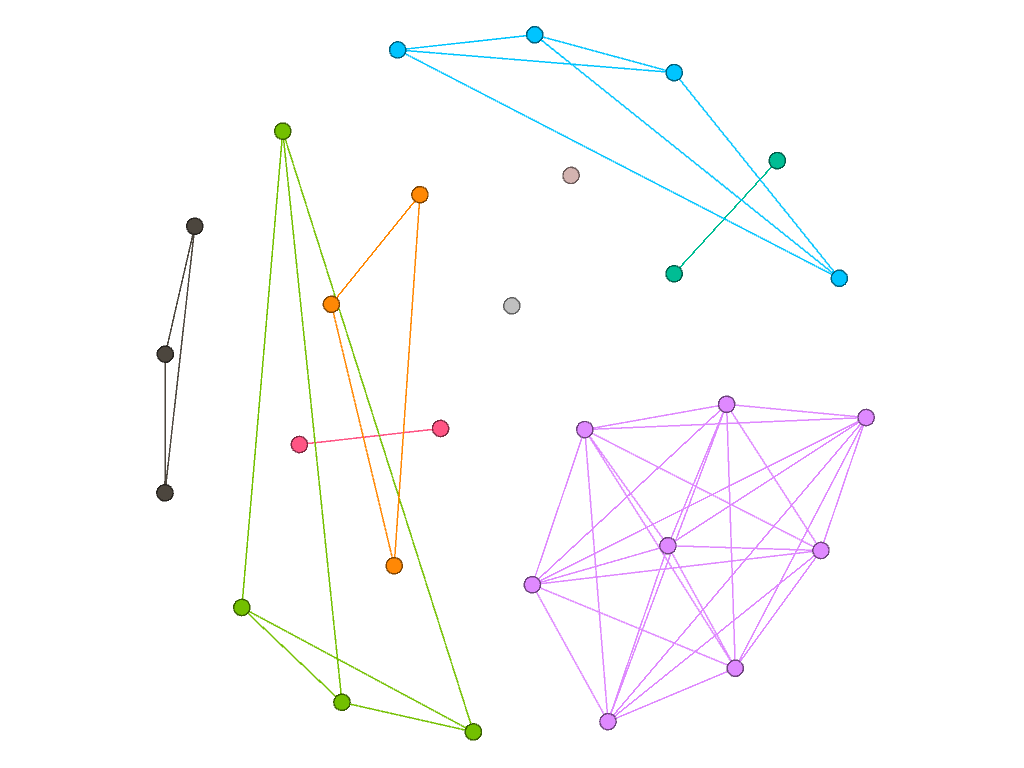
\includegraphics[width=1\textwidth]{img/parana-1998.png}
\caption{Grafo de coligações do Paraná em 1998.}
\label{grafo-parana-1998}
\end{figure}

Percebemos que esta modelagem não seria proveitosa, pois exigiria uma grande quantidade de grafos e mesmo assim não seria possível obter as informações desejadas para este trabalho. Desta forma, adotamos a abordagem 2.

A segunda abordagem apresenta ainda a opção de utilizar ou não grafos ponderados: o peso das arestas representaria em quantos estados os dois partidos participam de uma mesma coligação naquele ano.

Para exemplificar um dos motivos que nos levou a optar pelo uso de grafos ponderados, suponha um cenário com os partidos A, B e C, de forma que A e B sejam de esquerda e C seja de direita. Numa modelagem em um grafo não ponderado, se A faz aliança com B em quinze15 estados e com C em apenas um1 estado, esta informação seria representada através de duas arestas, uma de A para B e outra de A para C. Neste cenário, o grafo não seria uma representação adequada do comportamento do partido A.

%%%%%%%%%%%%%%%%%%%%%%%%%%%%%%%%%%%%%%%%%%%%%%%%%%%%%%%%%%%
\section{\texorpdfstring{\MakeUppercase{Restrições}}{}}
\label{proposta__restricoes}

A divisão ideológica dos partidos no Brasil não é trivial, no atual sistema político existem siglas com programas vagos e ideologias pouco claras, o que dificulta sua categorização dentro do espectro político. Com isso tornou-se inviável a categorização de alguns partidos presentes nos grafos apresentados neste trabalho.

Não é difícil perceber que existe falta de consenso dentro do cenário político como um todo em relação a como partidos se posicionam ou se encaixam no espectro político brasileiro, e essa categorização é inclusive foco de estudo de historiadores e sociólogos. Dessa forma, para a classificação dos partidos em \emph{esquerda}, \emph{direita}, \emph{centro} e as demais divisões ideológicas, optamos por categorizar de acordo com classificações encontradas em \todo{referencias}.

Por fim, entendemos que foge da proposta deste trabalho discorrer sobre questões socio-políticas a respeito dos dados apresentados, uma vez que estas questões podem ser melhor discutidas por estudiosos de outras áreas do conhecimento, como sociólogos, historiadores e cientistas políticos.

%%%%%%%%%%%%%%%%%%%%%%%%%%%%%%%%%%%%%%%%%%%%%%%%%%%%%%%%%%%
%%\section{\texorpdfstring{\MakeUppercase{Revisão da Bibliografia}}{}}
%%\label{proposta__revisao_bibliografia}

%%Algo light. Algum trabalho que possa ter motivado o nosso


%%%%%

%%%%%%%%%%%%%%%%%%%%%%%%%%%%%%%%%%%%%%%%%%%%%%%%%%%%%%%%%%%
\section{\texorpdfstring{\MakeUppercase{Objetivo Geral}}{}}
\label{proposta__objetivo-geral}

\todo{Talvez seja interessante apresentar algum contexto mais político, falar de informações interessantes q encontramos sei la}
Este trabalho propõe-se a utilizar o repositório de dados do \gls{TSE} para a construção de grafos referentes às informações de coligações partidárias no Brasil nos anos 1994 à 2014, com o objetivo de exibir métricas e visualizações que possam indicar existência de homofilia na formação de alianças políticas, isto é, se as coligações são formadas por partidos de ideologias semelhantes.

%%%%%%%%%%%%%%%%%%%%%%%%%%%%%%%%%%%%%%%%%%%%%%%%%%%%%%%%%%%
\section{\texorpdfstring{\MakeUppercase{Objetivos Específicos}}{}}
\label{proposta__objetivos-especificos}

%% Objetivos Específicos: ("pontual", em formato de lista. São pequenos objetivos para chegar/alcançar o objetivo geral do trabalho)
\subsection{Categorização dos partidos dentro do espectro político brasileiro}
\label{proposta__objetivos-especificos--categorizacao}

Avaliar os dados obtidos no repositório do \gls{TSE} e categorizar todos os partidos encontrados como sendo de esquerda, centro-esquerda, centro, centro-direita e direita. Esta categorização é feita inteiramente baseando-se nas informações apresentadas pelas referências utilizadas neste trabalho.

A classificação dos partidos dentro do espectro político nos permite entender quais partidos - em teoria - possuem afinidades ideológicas, gerando assim um meio de criarmos um referencial de como partidos se relacionariam se eles seguissem suas ideologias como base para criar coligações.

\subsection{Identificação de comunidades}
\label{proposta__objetivos-especificos--identificacao-comunidades}

Apresentar grafos para os anos de eleição estadual - 1994, 1998, 2002, 2006, 2010 e 2014 - e aplicar o algoritmo de modularização disponível no Gephi para a identificação de comunidades nestes grafos. Utilizando a categorização dos partidos dentro do espectro político, podemos analisar se as comunidades encontradas seguem algum padrão ideológico.

Optamos por tentar manter os grafos com duas comunidades, o que nos permite identificar se existe alguma divisão entre partidos de esquerda e direita.

\subsection{Análise e comparação dos grafos gerados}
\label{proposta__objetivos-especificos--analise-comparacao}

Utilizar a classificação de espectro político para analisar e comparar qual o padrão ideológico dos partidos presentes nas comunidades encontradas. Isso é feito através da geração de um segundo grafo para cada ano, no qual cada vértice é colorido de acordo com seu espectro político.

Esta abordagem provê uma facilidade na análise das comunidades, já que é possível comparar os grafos lado a lado e identificar relacionamentos entre os partidos, tamanho das comunidades e ideologia politica predominante em cada agrupamento de vértices.
%%%%%
\subsection{Informações apresentadas}
\label{proposta__objetivos-especificos--informacoes-apresentadas}

qual é o interesse em apresentar as informações sobre grau médio, coeficiente de clustering, ...
